\documentclass{article}
% if you need to pass options to natbib, use, e.g.:
%     \PassOptionsToPackage{numbers, compress}{natbib}
% before loading neurips_2019

% ready for submission% \usepackage{neurips_2019}

% to compile a preprint version, e.g., for submission to arXiv, add add the
% [preprint] option:
%     \usepackage[preprint]{neurips_2019}

% to compile a camera-ready version, add the [final] option, e.g.:
\usepackage[final]{neurips_2019}

% to avoid loading the natbib package, add option nonatbib:
%     \usepackage[nonatbib]{neurips_2019}

\usepackage[utf8]{inputenc} % allow utf-8 input
\usepackage[T1]{fontenc}    % use 8-bit T1 fonts
\usepackage{hyperref}       % hyperlinks
\usepackage{url}            % simple URL typesetting
\usepackage{booktabs}       % professional-quality tables
\usepackage{amsfonts}       % blackboard math symbols
\usepackage{nicefrac}       % compact symbols for 1/2, etc.
\usepackage{microtype}      % microtypography
\usepackage[pdftex]{graphicx}

\newcommand{\outOfCIPtcTrain}{94.7\%}
\newcommand{\outOfCIPtcTest}{94.1\%}

\title{Avocado Price Forecasting with Gaussian Processes}

% The \author macro works with any number of authors. There are two commands
% used to separate the names and addresses of multiple authors: \And and \AND.
%
% Using \And between authors leaves it to LaTeX to determine where to break the
% lines. Using \AND forces a line break at that point. So, if LaTeX puts 3 of 4
% authors names on the first line, and the last on the second line, try using
% \AND instead of \And before the third author name.

\author{%
  Anna Billiard  \\
  Data Science\\
  University of Michigan\\
  Ann Arbor, MI 48104 \\
  \texttt{annabill@umich.edu} \\
  \And Rohan Janakiraman \\
  Economics\\
  University of Michigan\\
  Ann Arbor, MI 48104 \\
  \texttt{rohanja@umich.edu} \\
  \AND Alex Brace \\
  Computer Science\\
  University of Michigan\\
  Ann Arbor, MI 48109 \\
  \texttt{braceal@umich.edu} \\
  \And Yi Zhang \\
  Computer Science and Data Science\\
  University of Michigan\\
  Ann Arbor, MI 48104 \\
  \texttt{zackLt@umich.edu} \\
}

\begin{document}
\maketitle
\begin{abstract}
Time series data often pose difficult, non-linear modeling problems and predictions tend to suffer from the inability to quantify uncertainty. We investigate alternatives to the traditional ARIMA methods of time series analysis by considering a Bayesian Gaussian process with a composite kernel function as the prior. The model fitted on historic avocado prices from 2015 to 2018 contained \outOfCIPtcTrain{} of the sample/observed data and \outOfCIPtcTest{} of the out-of-sample/unobserved true data, despite having a fairly minimal feature space. This paper attempts to establish that for price prediction problems, Gaussian processes are an effective and interpretable model choice. 
\end{abstract}

\section{Introduction}
Gaussian processes (GP) present an opportunity to fit heavily non-linear models using Bayesian inference in a way that makes quantifying uncertainty extremely easy. For instance, as a direct result of its Bayesian nature, GPs can generate posterior predicate check (PPC) intervals for credibility ranges enclosing the predictions. The uncertainty quantification distinguishes GPs from many other machine learning approaches.

As a demonstration, we fit a Gaussian process model to historic avocado prices from 2015 to 2018. We used several optimization techniques such as Broyden–Fletcher–Goldfarb–Shanno (BFGS) and random search to tune model hyperparameters. The resulting model performed satisfactorily despite having data limited in quantity and quality. The 95\% PPC intervals we generated encompassed most of the true data points in our test dataset, validating our model and the use of GPs in price forecasting.

\section{Data}
   Hass avocados are one of the primary types of avocados sold in the United States. The non-profit organization Hass Avocado Board (HAB) collected the avocado price data through Information Resources' channels with "multi-outlet stores... based on actual retail sales of Hass avocados" [1]. HAB published the dataset including weekly average prices for individual Hass avocados sold in grocery stores segmented by organic and conventional and by state, as well as nationally and regionally aggregated averages [2].
   
    With 161 weeks of data and 18,249 individual observations (averages for different places and types of avocado) from January 2015 through March 2018, the dataset spans a wide range of areas. Figure 1 shows a histogram of observations. The bi-modality results from the difference between organic and conventional avocado prices. Note the right tail. Our hypothesis is that the tail could be attributed to two separate things: the year 2016 and 2017 having high outliers (see figure 2), and the fact that some states have higher avocado prices in general (see California and Connecticut in Figure 6, appendix A). 
    
    Figure 2 shows a slight upward shift in prices in 2017 (by approximately \$0.15). We attribute this uptick to a growers’ strike in Mexico and a concurrent drought in California [3].
    
    For our model, we chose to only use the prices of organic avocado in West Texas and New Mexico, a predefined region in the dataset. There are three reasons for the choice of location. First, although it may seem that the U.S. average prices would be the best choice, it turns out to contain some quite abnormal price points with wide fluctuations that would make modeling unnecessarily challenging for the demonstration. Second, West Texas and New Mexico, in particular, have easy access to avocados while not having a lot of avocado production [4]. Additionally, the choice to work only on organic avocados lies in the fact that its larger variance would better highlight the pattern fitting ability of GP (see Figure 3 and Table 3 in Appendix A).
    
\begin{figure}[!htb]
\begin{minipage}{0.48\textwidth}
    \centering
    \includegraphics[width=1\linewidth]{images/price-histogram.png}
    \caption{Right-skewed bi-modal distribution of \\avocado prices.}\label{Fig:Data1}
\end{minipage}\hfill
\begin{minipage}{0.48\textwidth}
    \centering
     \includegraphics[width=1\linewidth]{images/Avocado-Price-Dist-Updated.png}
    \caption{Spike in summer 2017 prices due to drought and growers strike.}\label{Fig:Data2}
\end{minipage}
\end{figure}

\begin{figure}[h!]
  \centering
  \includegraphics[width=1\linewidth]{images/Avocado-Price-Range-Region-Flipped.png}
  \caption{Price distribution of organic avocados vs. conventional avocados in various areas.}\label{Fig:Data3}
\end{figure}

\section{Methods}
\subsection{Definition of Gaussian Process}
 A Gaussian process fits a non-parametric model that assumes observations in the data set follow a multivariate-normal (MVN) distribution with a mean function and a kernel function to define the covariance matrix. The initial kernel and mean function define the MVN prior, while our training data are used to model the data likelihood function. The prior and likelihood functions are then used to make Bayesian updates to arrive at a conjugate posterior model. We define the GP model below as adapted from \textit{Gaussian processes for machine learning} [5].

Let $\mathcal{X}$ be the set of weekly enumerated time intervals $\textbf{X}$, where $\textbf{X} = (x_1, ..., x_n)$ is the indices of weekly avocado price observations.

Let $(f(x_1), ..., f(x_n))$ s.t. $f(x_i) \in \mathbb{R}$ be the time series of avocado price observations.

Define mean function $\mu : \mathcal{X} \rightarrow \mathbb{R}^n$ where $\mu(\textbf{X}) = \mathbb{E}[f(\textbf{X})]$. It is often the mean of the training set if the prior belief holds the variable mean(s) to be stationary, as in our case.

Define covariance function $\kappa : \mathcal{X} \times \mathcal{X} \rightarrow \mathbb{R}^{n\times n}$ where $\kappa(\textbf{X}, \textbf{X}^\prime) = \mathbb{E}[(f(\textbf{X}) - \mu(\textbf{X}))(f(\textbf{X}^\prime) - \mu(\textbf{X}^\prime))]$.

We define a Gaussian process as: $(f(x_1), ..., f(x_n)) \sim MVN(\mu(\textbf{X}), \kappa(\textbf{X}, \textbf{X}^\prime))$.

\subsection{Kernel Function Selection}

We found that the most important part of specifying our model to be kernel function selection. The kernel function encodes prior knowledge about the data. From exploratory data analysis, we concluded that the avocado price series has a cyclic pattern over a one year period. To account for both the seasonal trend and the autoregressive correlation of neighboring data points, we decided to use exponential sine squared (ESS) kernel function, a sinusoidal variant of the common radial basis function (RBF) kernel, equation (1), implemented by scikit-learn [10]. This kernel has two hyperparameters, $p > 0$ which accounts for the periodicity and $l > 0$ which accounts for the decay of importance between far away points.

\begin{equation}
\centering
\kappa(x_i, x_j)_{ESS} = exp\bigg\{\frac{-2}{l^2}sin^2(\frac{\pi}{p}\cdot \|x_i - x_j\|_2) \bigg\}
\end{equation}

For robustness, we also added the rational quadratic (RQ) kernel function, equation (2). This kernel accounts for medium term irregularities according to scikit-learns documentation [6]. Introducing this kernel helps account for the irregular price spikes such as the one in 2017. This kernel also has two hyperparameters, $l > 0$ which has the same effect as above and $\alpha > 0$ which accounts for relative weighting of small and large scale variations [7].

\begin{equation}
\centering
\kappa(x_i, x_j)_{RQ} = \bigg(1 + \frac{\|x_i - x_j\|_2^2}{2\alpha l^2}\bigg)^{-\alpha}
\end{equation}

Lastly, we define a white noise (WN) kernel function which acts as a regularizer in our model, equation (3). This kernel works by adding a constant value $\epsilon$ to the diagonal of the covariance matrix i.e. Tikhonov regularization [9]. Here epsilon is learned from the global noise in the training data.

\begin{equation}
\centering
\kappa(x_i, x_j)_{WN} = \mathbb{I}(x_i = x_j) \cdot \epsilon
\end{equation}

Combining equations (1-3), we define a composite kernel function, equation (4), that we used to model and forecast the avocado prices. Note, the summation of kernel functions is still a valid differentiable kernel function since this operation effectively makes the covariance matrix in MVN a summed matrix with non-negative diagonal values. For our prior belief, we set the hyperparameters in the following fashion: length scales are all 20 to take into account of 20 weeks as short term influences/trends. Periodicity to be 365 to reflect yearly trends. A white noise level of .13 as the variance close to that of the average organic avocado price for all regions. A .8 multiplier for the RQ kernel function (which adds fluctuations to the ESS kernel function) since we believe the overall trend outweights the intra-year fluctuations. (The hyperparameters do not need to be precise since the model automatically tunes and restarts at random locations in the hyperparameter space.)

\begin{equation}
\centering
\kappa(x_i, x_j) = \kappa_{ESS} + 0.8\cdot \kappa_{RQ} + \kappa_{WN}
\end{equation}

\subsection{Model Implementation}

To implement our model, we used scikit-learn, a Python library, which has several built-in kernel functions that we arranged in a linear combination. To optimize kernel hyperparameters we employed the limited memory BFGS optimizer implemented by scikit-learn [6], which optimizes kernel hyperparameters during model fitting by maximizing the log-marginal likelihood using a gradient ascent iteration [8]. To avoid getting trapped in local optima in the hyperparameter space (such as a high noise model), we restart the optimizer a fixed number of times (typically 10). The first run of the optimizer is initialized with a best guess prior estimate and subsequent optimizations are initialized via a random sample from the hyperparameter space.

To reduce over-fitting to the training data, we regularize our model using Tikhonov regularization. This is achieved by the addition of a white noise kernel to our kernel function which models the global noise in the training data and adds it to the MVNs covariance matrix diagonal.

\section{Results}

\begin{equation}
\centering
\kappa(x_i, x_j) = \kappa(lengthScale=4.57, periodicity=337)_{ESS} + \\ 0.0497\cdot \kappa(alpha=1e+05, lengthScale=21.7)_{RQ} + \kappa(noiseLevel=0.0158)_{WN}
\end{equation}

We obtain the fitted model with the above hyperparameters. It turns out the long term fluctuations would have a length scale of 4.57, short term to have one of 21.7, giving us a time window for the long-term and short-term price fluctuations. The periodicity is 337 instead of 365, likely influenced by the actual crop year for our data. The noise level of .0158, much lower than the variance in the training data, suggests the model is able to find a good fit. A large value of alpha makes the short term RQ kernel function approach the ESS function, meaning the model finds the long term trend is much more meaningful. Thus, with the combination of the RQ and the ESS kernels, we are able to account for both long and short term periodic trends which explains why this model performed so well off-sample.

To assess model fit, we split our data into training and testing sets with an 80-20 split into each category respectively. The training data runs from January 1, 2015 to July 31, 2017 while the testing data runs from August 06, 2017 to March 18, 2018.

Figure 4 shows our model against the training and test data. The dark blue band represents the GP uncertainty and the light blue band represents the 95\% PPC interval. Our model showed excellent results with \outOfCIPtcTest{} of testing data and \outOfCIPtcTrain{} of the training data within the 95\% PPC interval. The fact that the training and testing sets showed very similar prediction accuracy is evidence that our model generalized well to off-sample data, proving the success of the regularization. As a comparison, we have included Figure 5, which shows the original data and a regression done using splines. Evidently, the GP model fits the volatility in the data much better.

The 95\% PPC interval also demonstrates the utility of a GP model. Not only can we forecast a price on a particular week but we can also provide our uncertainty of the estimate with mathematically sound credibility. 

\begin{figure}[h!]
  \centering
  \includegraphics[width=1.1\linewidth]{images/gp-WestTexNewMexico-results.png}
  \caption{Gaussian process regression results for organic avocado prices in the West Texas/New Mexico region. The training and testing data are shown in black and red, respectively. The regression line is shown in orange and the GP uncertainty (one standard deviation) and 95\% PPC interval are depicted by the dark blue band and light blue band, respectively. The 95\% PPC interval accounts for \outOfCIPtcTest{} of testing data and \outOfCIPtcTrain{} of training data.}
\end{figure}

\begin{figure}[h!]
  \centering
  \includegraphics[width=1\linewidth]{images/baseline-WestTexNewMexico-results.png}
  \caption{Standard regression results for organic avocado prices in the West Texas/New Mexico region. The regression line is shown in blue and the 95\% confidence interval is depicted by the grey bands.}
\end{figure}

\begin{table}[h!]
\centering
\begin{tabular}{ |p{2cm}||p{2cm}|p{2cm}|p{2cm}| }
 \hline
 \multicolumn{4}{|c|}{Gaussian process model performance} \\
 \hline
 Data set& RMSE & $R^2$ & Accuracy\\
 \hline
 Train &  0.109  &  0.874  & \outOfCIPtcTrain{} \\
 Test  &  0.295  & -0.796  & \outOfCIPtcTest{} \\
 \hline
\end{tabular}
\caption{Reported statistics for GP model performance in the West Texas/New Mexico region. (Accuracy: Percentage of Test Data within PPC Interval)}
\end{table}



Table 1 above has relevant statistics. The quantity $R^{2}$ is defined as $1 - \frac{\sum{(y_i - \hat{y})}^2}{\sum(y_i - \bar{y})^2}$, or in other words one minus the variance of our model divided by the variance of the data itself. Note that this can be negative if the model variance is higher than the data variance or because of systematic bias i.e. overfitting. Our $R^{2}$ value for the testing set is indeed negative. It resulted from consistently lower predictions for the year of 2017 rather than overfitting (2017 is influenced by the drought and strike as mentioned above compared to the previous two years). Nevertheless, our model captures the trend of the data well and is able to contain most real prices with credible intervals. Root mean squared error (RMSE) was calculated by comparing our models predicted price of organic avocados in West Texas/New Mexico to the true values. An RMSE of 0.295 in the test set reveals that our model did fairly well at explaining the variance of the test set, though this model leaves lots of room for improvement (see discussion). 

Our model predicted mean for the test period was 1.655 and the true mean over this time was 1.887. The optimized hyperparameter for the ESS kernel function that described the periodicity  was 337, which is about the same as the number of days in a year. This is not coincidental, as plants are heavily dependent on the yearly cycle of seasons, highlighting the interpretability of GP. 

\section{Discussion}
Some drawbacks to our analyses should be noted. There are many other factors that drive avocado prices other than the price alone. Our data do not account for factors such as tariffs, farm subsidies, growers’ strikes (possibly with their own cyclical patterns), persecution of illegal immigrants who make up much of the agricultural workforce in the U.S., and the climate crisis all affect the market for avocados [11]. To illustrate the need to include such factors, consider the aforementioned Mexican growers’ strike, which contributed to the price spike that we observed in the 2017 data. After doing more research, we found that these strikes are a semi-regular event, as there was also a strike in November 2018 which disrupted shipments from Mexico [12]. The regularity of these strikes is likely tied to the length of the union contracts the avocado growers have with APEAM, an avocado industry group that manages the “Avocados from Mexico” brand. Future research could be done to ascertain the magnitude of the price shocks such strikes cause as well as their seasonality. 

Future work along these lines would ideally culminate in a higher-dimensional GP model. This model would have several more ESS kernels to model more types of periodicity in the dataset. This would allow us to model for several of those other factors discussed above in addition to the year, which could be useful when we procure the aforementioned additional data.

Despite the low dimensionality of our data, Gaussian processes have important positives. Gaussian process regression has an advantage over loss-function based models, since it learns a generative model of the data that can be used to provide credible intervals for predictions. In loss-function based models, we do not have any knowledge of the stability or uncertainty around predictions. Overall, GP models are very interpretable and provide robust predictions for off-sample data.

In addition, for low dimensional data, as in the case of Avocado prices, optimizing hyperparameters for GPs can be done very efficiently by taking advantage of gradient information implicit in the kernel function. This is a significant advantage over loss-function based black box models such as neural networks, which  resort to grid search, Bayesian optimization, etc. for optimizing hyperparameters.

\section{Conclusion}
    Overall, our Gaussian process model performed quite well. The component kernel functions ended up with hyperparameters that reflected concrete aspects of the data, such as the periodicity of approximately one year. Though our RMSE for the test set was nearly 0.3, we attribute this to the variance of the data set itself (see table 3) as well as the low-dimensionality of our model. Additionally, the accuracy of the 95\% PPC indicates that our model works quite well on the data as a whole.
    
    We achieved great results of using Gaussian processes to fit a Bayesian model to the avocado price dataset. Learning a model that did not overfit to the data and had predictive power is a clear indication that Gaussian processes were appropriate in this case. 
    
\section{Contributions}
    Anna Billiard - Research into Gaussian processes, doing Gaussian processes with R, kernel functions; the presentation slides and presentation to the class; abstract, introduction, data, conclusion, the bulk of discussion, and parts of methods and results sections of paper; editing of the overall paper.
    
    Alex Brace - Research into Gaussian processes and how they work; the data segmentation in Python; fitting, tuning and visualizing Gaussian process models in Python; built avocado Python package for rapidly testing GP models; the methods section and part of the discussion section in the report.
    
    Rohan Janakiraman - Exploratory data analysis in R, calculated summary statistics, most of the figures, tables 2 and 3 in appendix A, all of appendix B, references section, some of the discussion section, the research behind the price spike in 2017, organized project materials, some editing.  
   
    Yi Zhang - Research and coding Gaussian processes in R and Python, kernel functions; studying Gaussian process papers and reports by Hass Avocado Board; code repository management; evaluating the model results; writing parts of the Discussion of the paper; overall editing of the paper.


\section*{References}

\small

[1] Carman, Hoy F., Tina L. Saitone, and Richard J. Sexton. (2013). Five-year evaluation of the Hass Avocado Board’s promotional programs: 2008-2012. \textit{Hass Avocado Board}.

[2] Kiggins, J. (2017). Avocado Prices: Historical data on avocado prices and sales volume in multiple US markets. \textit{Kaggle}.

[3] Perez, M. G., \&\ Durisin, M. (2017). Avocado Prices Are Skyrocketing. \textit{Bloomberg}.

[4] Nesbitt, M., Stein, L., \&\ Kamas, J. (2015). Avocados. \textit{Texas A&M AgriLife Extension Service}.

[5] Williams, C. K., \&\ Rasmussen, C. E. (2006). Gaussian processes for machine learning. \textit{MIT press}.

[6] Pedregosa, F. et. al. (2011). Scikit-learn: Machine Learning in Python. Gaussian Process Regressor. \textit{Journal of Machine Learning Research, 12}, 2825 - 2830. 

[7] Duvenaud, D. (2014). Automatic model construction with Gaussian processes (Doctoral dissertation, \textit{University of Cambridge}).

[8] Liu, D. C., \&\ Nocedal, J. (1989). On the limited memory BFGS method for large scale optimization. \texit{Mathematical programming, 45}(1-3), 503-528.

[9] Golub, G. H., Hansen, P. C., \&\ O'Leary, D. P. (1999). Tikhonov regularization and total least squares. \textit{SIAM Journal on Matrix Analysis and Applications, 21}(1), 185-194.

[10] Pedregosa, F. et. al. (2011). Scikit-learn: Machine Learning in Python. Exp Sine Squared. \textit{Journal of Machine Learning Research, 12}, 2825 - 2830. 

[11] Rooney, K. (2019). Avocados will probably get more expensive under Trump’s Mexico tariffs. \textit{CNBC}.

[12] Chiwaya, N. (2018). Can’t get your hands on avocados lately? Here’s why. \textit{NBC News}. 


\newpage
\appendix
\section{Avocado Data Summary Statistics \& State-by-State Price Breakdown}

\begin{table}[h!]
\centering
\begin{tabular}{ |p{2.0 cm}||p{2.0 cm}|p{2.2 cm}|p{2.2 cm}|p{2.2 cm}|p{2.4 cm}|}
 \hline
 \multicolumn{6}{|c|}{Data Summary Statistics} \\
 \hline
 Variable & Num of Obs. & Mean & Std Dev & Range & IQR \\
 \hline
 \textit{AveragePrice} &  18249  &  1.406 & 0.402 & [0.44, 3.25] & [1.10, 1.66]   \\
 \textit{Total Volume} &  18249  & 850644 & 3453545 & [85, 62505647] & [10839, 432962]  \\
 \textit{4046} & 18249 & 293008 & 1264989 & [0, 22743616] & [854, 111020] \\
 \textit{4225} & 18249 & 295155 & 1204120 & [0, 20470573] & [3009, 150207] \\
 \textit{4770} & 18249 & 22840 & 107464.1 & [0, 2546439] & [0, 6243] \\
 \textit{Total Bags} & 18249 & 239639 & 986242.4 & [0, 19373134] & [5089, 110783]\\
 \textit{Small Bags} & 18249 & 182195 & 746178.5 & [0, 13384587] & [2849, 83338] \\
 \textit{Large Bags} & 18249 & 54338 & 243966 & [0, 5719097] & [127, 22029]\\
 \textit{XLarge Bags} & 18249 & 3106.4 & 17692.89 & [0.0, 551693.7] & [0.0, 132.5] \\ 
 \hline
\end{tabular}
\caption{The variables \textit{4046}, \textit{4225}, \textit{4770} denote the total number of avocados with PLU 4046, PLU 4225 and PLU 4770 sold respectively. PLU means 'Price Look Up' code and they have been used by supermarkets to make inventory control easier. }
\end{table}

\begin{table}[h!]
\centering
\begin{tabular}{|p{2.4 cm}||p{2.4 cm}|p{2.4 cm}|p{2.4 cm}|p{2.4 cm}|}
\hline
 \multicolumn{5}{|c|}{Conventional Avocado Prices vs. Organic Avocado Prices} \\
 \hline
  Type & Num of Obs. & Mean & Variance & IQR \\
 \hline
 Organic & 9123 & 1.654 & 0.132 & [1.42, 1.87]\\
 Conventional & 9126 & 1.158 & 0.069 & [0.98, 1.32]\\
 \hline
\end{tabular}
\caption{Comparison of average avocado prices for both conventional and organic avocados using the variable \textit{AveragePrice}.}
\end{table}

\begin{figure}[h!]
  \centering
  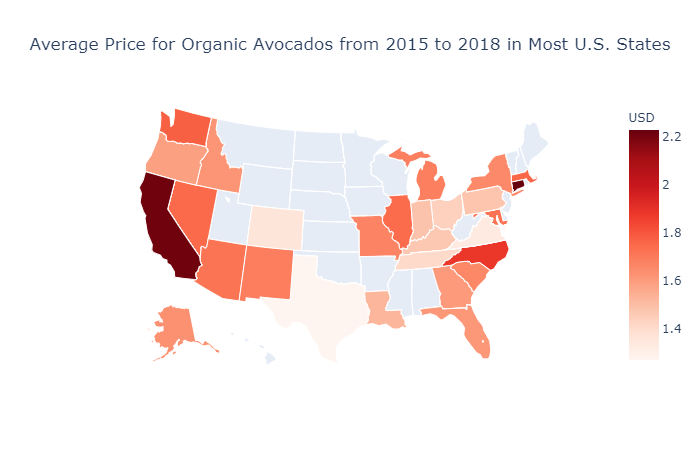
\includegraphics[width=1\linewidth]{images/price_by_states.png}
  \caption{Average prices in most U.S.}\label{Fig:Data3}
\end{figure}

\newpage
\section{Avocado Price Distribution Plots, By Year}
\begin{figure}[!htb]
\begin{minipage}{0.48\textwidth}
    \centering
    \includegraphics[width=1\linewidth]{images/Avocado-Prices-2015.png}
    \label{Fig:Data5}
\end{minipage}\hfill
\begin{minipage}{0.48\textwidth}
    \centering
     \includegraphics[width=1\linewidth]{images/Avocado-Prices-2016.png}
    \label{Fig:Data6}
\end{minipage}
\end{figure}

\begin{figure}[!htb]
\begin{minipage}{0.48\textwidth}
    \centering
    \includegraphics[width=1\linewidth]{images/Avocado-Prices-2017.png}
    \label{Fig:Data5}
\end{minipage}\hfill
\begin{minipage}{0.48\textwidth}
    \centering
     \includegraphics[width=1\linewidth]{images/Avocado-Prices-2018.png}
    \label{Fig:Data6}
\end{minipage}
\end{figure}

\end{document}